
\documentclass[border=6pt]{standalone}
\usepackage[T1]{fontenc}
\usepackage{helvet}
\renewcommand{\familydefault}{\sfdefault}
\usepackage{amsmath}
\usepackage{graphicx}
\usepackage{xcolor}
\usepackage{enumitem}
\usepackage{tikz}
\usetikzlibrary{positioning,arrows.meta}

% ---------- colours (one per panel) ----------
\definecolor{cProp}{HTML}{4A90C2}   % blue
\definecolor{cOpt}{HTML}{E0B03A}    % yellow
\definecolor{cSweep}{HTML}{5AAE61}  % green
\definecolor{cAnn}{HTML}{8C7BC4}    % purple
\definecolor{cTewi}{HTML}{D9534F}   % red
\definecolor{cArrow}{HTML}{8B5A1E}  % brown arrows

% ---------- sizes (change here) ----------
\newlength{\panelW}\setlength{\panelW}{4.3cm}   % panel text width
\newlength{\panelH}\setlength{\panelH}{8.6cm}   % panel height

% ---------- helpers ----------
\setlist[itemize]{leftmargin=1.1em, itemsep=1pt, topsep=2pt, parsep=0pt, label=\textbullet}
\newcommand{\paneltitle}[1]{{\centering\large\bfseries #1\par}\vspace{4pt}\raggedright}
\newcommand{\idaeslogo}{%
  \par\vspace{6pt}\centering{\LARGE\bfseries IDAES-PSE}\\[-3pt]
  {\color{red!80!black}\rule{2.2cm}{1.4pt}}\par\vspace{4pt}}
% map pin drawn in TikZ (no extra packages needed)
\newcommand{\pin}[1]{\tikz[baseline=-1pt]{%
  \fill[#1] (0,-0.05) -- (-0.13,0.20) arc[start angle=180,end angle=0,radius=0.13] -- cycle;
  \fill[white] (0,0.21) circle (0.05);}}

\tikzset{
  panel/.style={draw=#1!70, fill=#1!8, rounded corners=6pt, line width=0.9pt,
                inner sep=5pt, anchor=north west},
  flow/.style={-{Triangle[length=7pt,width=10pt]}, line width=5pt, cArrow}
}

\newcommand{\panelbox}[1]{\begin{minipage}[t][\panelH][t]{\panelW}\raggedright #1\end{minipage}}

\begin{document}
\begin{tikzpicture}[node distance=0.55cm]

% ---------------- 1. Properties ----------------
\node[panel=cProp] (p1) {\panelbox{%
  \paneltitle{Properties}
  \begin{itemize}
    \item Helmholtz equation of state models
    \item R-515B, R-1234yf and R-134a
    \item Implemented in IDAES-PSE
  \end{itemize}
  \idaeslogo
  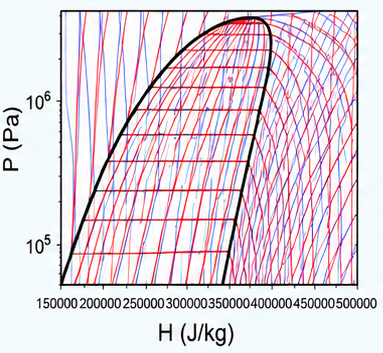
\includegraphics[width=\linewidth]{ph_diagram}
}};

% ---------------- 2. Max COP ----------------
\node[panel=cOpt, right=of p1.north east, anchor=north west] (p2) {\panelbox{%
  \paneltitle{Max COP}
  \begin{itemize}
    \item Single stage and cascade configurations
    \item Optimization with IDAES-PSE \& IPOPT
  \end{itemize}
  \idaeslogo
  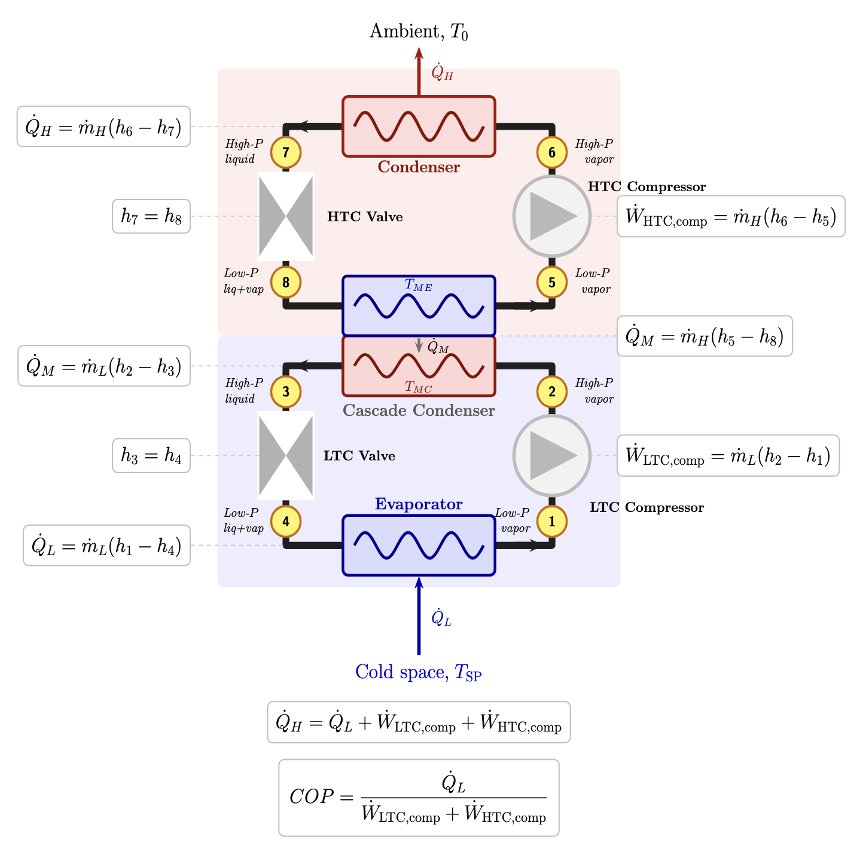
\includegraphics[width=\columnwidth]{cascade_schematic}
}};

% ---------------- 3. COP vs ambient sweep ----------------
\node[panel=cSweep, right=of p2.north east, anchor=north west] (p3) {\panelbox{%
  \paneltitle{COP vs Ambient Sweep}
  \begin{itemize}
    \item COP as a function of ambient temperature
    \item R-515B, R-1234yf and R-134a
    % \item Single stage and cascade configurations
  \end{itemize}
  \vspace{30pt}
  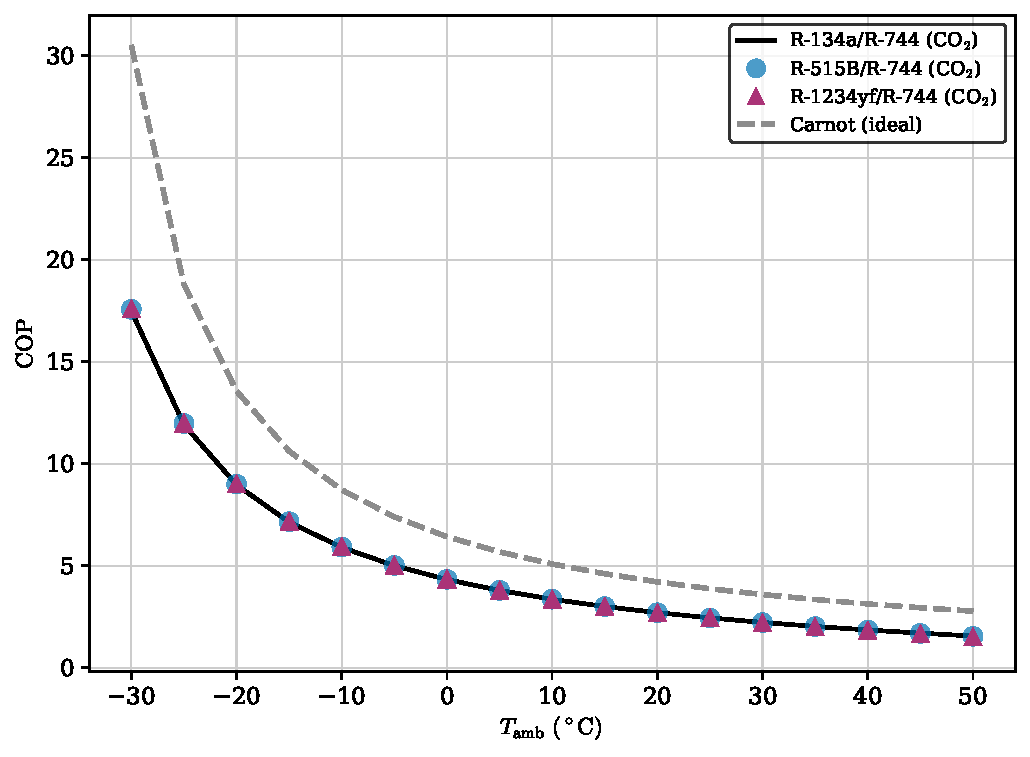
\includegraphics[width=\linewidth]{cascade_cop_vs_ambient}
}};

% ---------------- 4. Annualized data ----------------
\node[panel=cAnn, right=of p3.north east, anchor=north west] (p4)
{\panelbox{%
  \paneltitle{Annualized Data}
  \begin{itemize}
    \item Detailed model in Modelica
    \item Annual performance in 4 cities using TMY3 weather data
    % \item Single stage and cascade configurations
  \end{itemize}
  \par\vspace{6pt}\centering{\LARGE\bfseries Modelica}\par\vspace{4pt}
  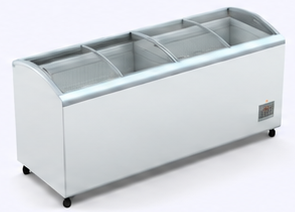
\includegraphics[width=0.85\linewidth]{freezer}\par\vspace{4pt}
  {\small TMY3 weather data}\par\vspace{15pt}
  {\scriptsize
   \begin{tabular}{@{}c@{\hspace{4pt}}c@{\hspace{4pt}}c@{\hspace{4pt}}c@{}}
     \pin{red!80!black} & \pin{blue!70!black} & \pin{green!55!black} & \pin{orange!90!black}\\
     Chicago & Atlanta & San Diego & Tucson
   \end{tabular}}
}};
\vspace{60pt}
% ---------------- 5. Lifetime emissions ----------------
\node[panel=cTewi, right=of p4.north east, anchor=north west] (p5) {\panelbox{%
  \paneltitle{Lifetime Emissions}
  \begin{itemize}
    \item Total equivalent warming impact (TEWI) over 15 years
  \end{itemize}
  \vspace{10pt}
  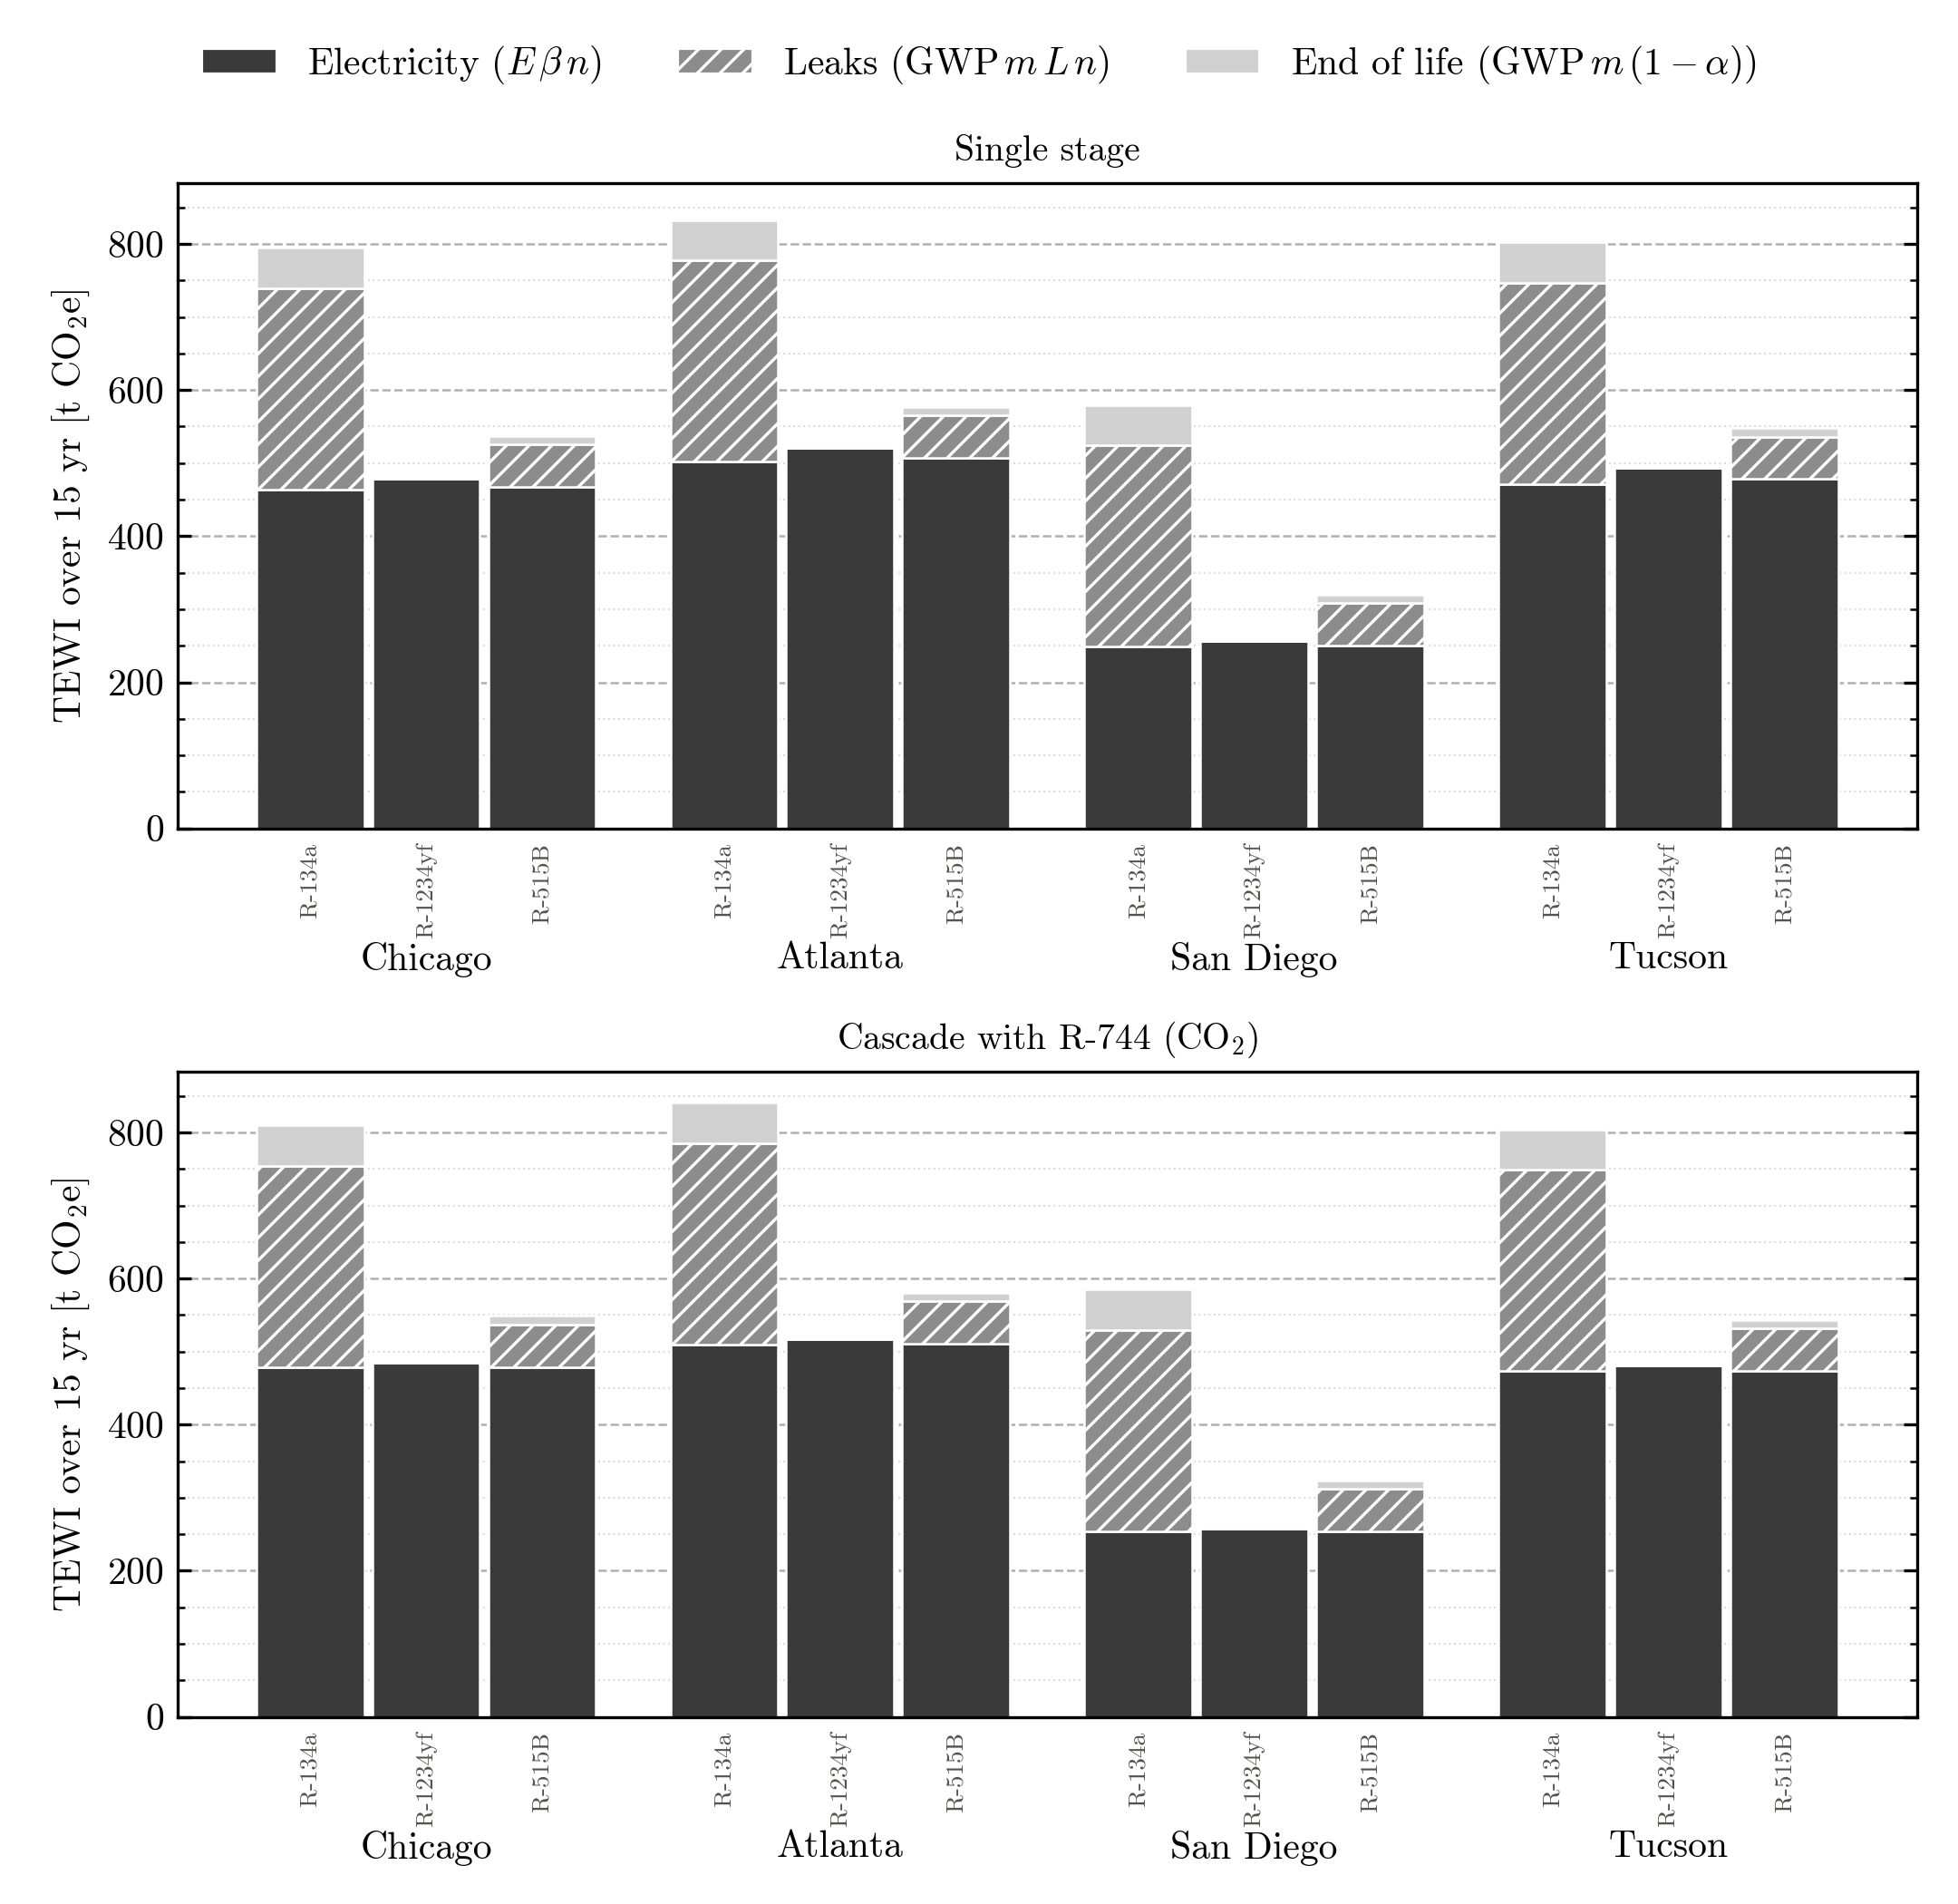
\includegraphics[width=\linewidth]{tewi_figure_L10_n15_cascade100.png}
}};

% ---------------- arrows between panels ----------------
\foreach \a/\b in {p1/p2, p2/p3, p3/p4, p4/p5}
  \draw[flow] ([xshift=-1pt]\a.east) -- ([xshift=1pt]\b.west);

\end{tikzpicture}
\end{document}
